\documentclass[frontgrid]{flacards}
\usepackage{graphicx}
\usepackage{color}

\definecolor{light-gray}{gray}{0.75}

\newcommand{\frontcard}[1]{\textcolor{light-gray}{\colorbox{light-gray}{$#1$}}}
\newcommand{\backcard}[1]{#1} 

\newcommand{\flashcard}[1]{% create new command for cards with blanks
    \card{% call the original \card command with twice the same argument (#1)
        \let\blank\frontcard% but let \blank behave like \frontcard the first time
        #1
    }{%
        \let\blank\backcard% and like \backcard the second time
        #1
    }%
}

\begin{document}

\pagesetup{2}{4} 

\card{
  What do we do here?\\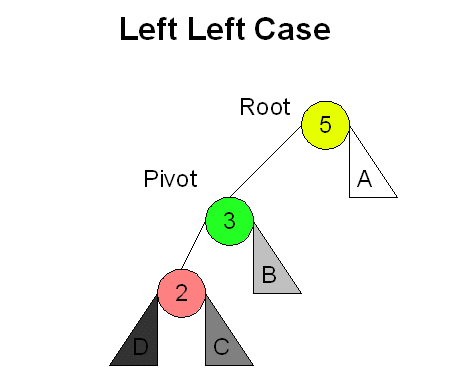
\includegraphics[height=0.8\cardheight]{images/left-left}
}{
  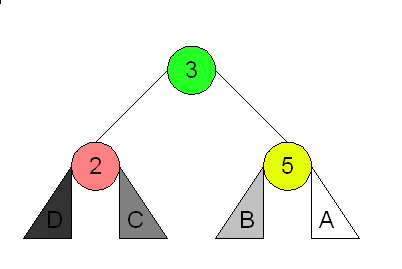
\includegraphics[height=0.8\cardheight]{images/left-left-out}
}

\card{
  What do we do here?\\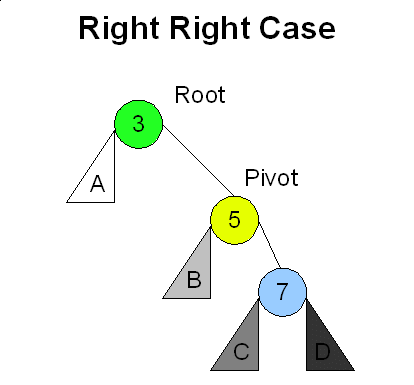
\includegraphics[height=0.8\cardheight]{images/right-right}
}{
  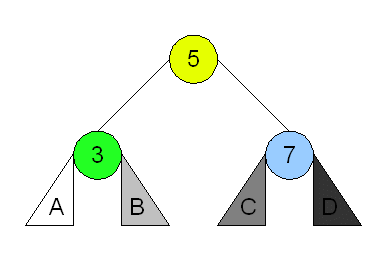
\includegraphics[height=0.8\cardheight]{images/right-right-out}
}

\card{
  What do we do here?\\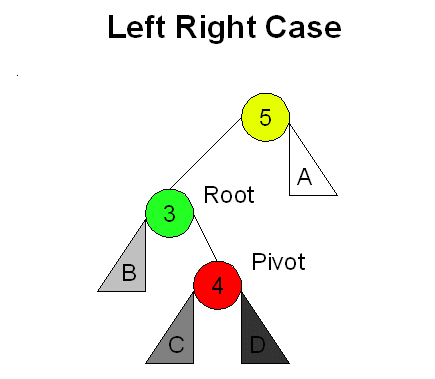
\includegraphics[height=0.8\cardheight]{images/left-right}
}{
  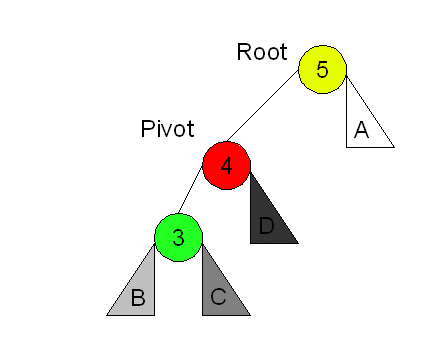
\includegraphics[height=0.8\cardheight]{images/left-right-mid}\\
  Then a left-left!
}

\card{
  What do we do here?\\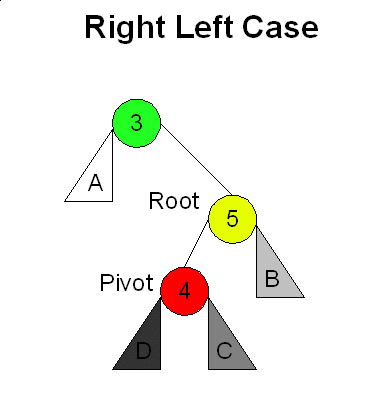
\includegraphics[height=0.8\cardheight]{images/right-left}
}{
  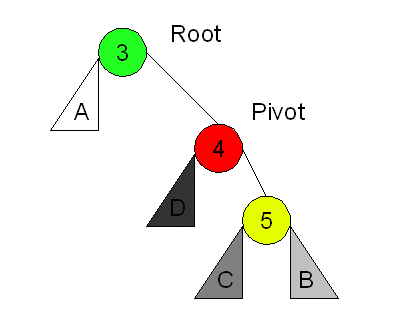
\includegraphics[height=0.8\cardheight]{images/right-left-mid}\\
  Then a right-right!
}

\card{
  What does a Depth First Search use?
}{
  A stack!
}

\card{
  What does a Breadth First Search use?
}{
  A queue!
}

\card{
  What is the running time of Dijkstra's algorithm?
}{
  $O(E + V\log(v))$
}

\card{
  What's the running time of a depth first search when the graph is an adjacency
  matrix?
}{
  $O(V^2)$ since finding neighbours takes $O(V)$ time.
}

\card{
  What's the running time of a depth first search when the graph is an adjacency
  list?
}{
  $O(V + E)$
}


\end{document} 